% 可见光谱
% 光谱|颜色|波长|视网膜

可见光的波长范围在大约 400nm 到 700nm 之间. 各个波长对应的颜色如\autoref{VisSpt_fig1}, 图中我们进一步将可见光根据波长划分为红,橙,黄,绿,蓝,紫几个区间.

\begin{figure}[ht]
\centering

\includegraphics[width=14cm]{./figures/VisSpt_1.png}
\caption{电脑生成的标准可见光谱(图片来自维基百科)} \label{VisSpt_fig1}
\end{figure}

\subsection{人眼和显示器}
我们知道人眼可以识别不同的波长是因为我们视网膜上有三种不同的感光细胞, 它们分别主要感受红, 绿, 蓝三种波长的光, 再根据这三种信号的大小在大脑中还原出不同的颜色. 显示器也根据人眼的这种特性对每个像素设置了红, 绿, 蓝三种颜色\footnote{一些动物的感光细胞不一样, 所以当它们看屏幕是, 看到的颜色可能与我们不同.}.

当电脑储存一张彩色图片时, 每个像素会被储存为 red, green, blue (或记为 RGB) 三个数, 每个数一般取 $0$ 到 $255$ 的整数, 有时候也取 $0$ 到 $1$ 的实数. \autoref{VisSpt_fig1} 中, RGB 三个分量的大小如\autoref{VisSpt_fig2} 所示, 这可以反映出人眼中三种受体对不同波长的敏感程度.

\begin{figure}[ht]
\centering
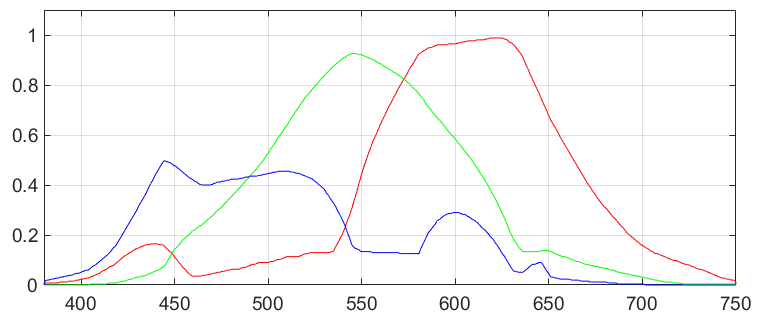
\includegraphics[width=12cm]{./figures/VisSpt_2.png}
\caption{RGB 三个分量} \label{VisSpt_fig2}
\end{figure}
